\section{Overall System Description}
\label{sec:overall_system_description}


\subsection{Description}

% Slayt 45. sayfa, buna eklem cikarma yapabiliriz isteginiz dogrultusunda...
\begin{figure}[h]
    \centering
    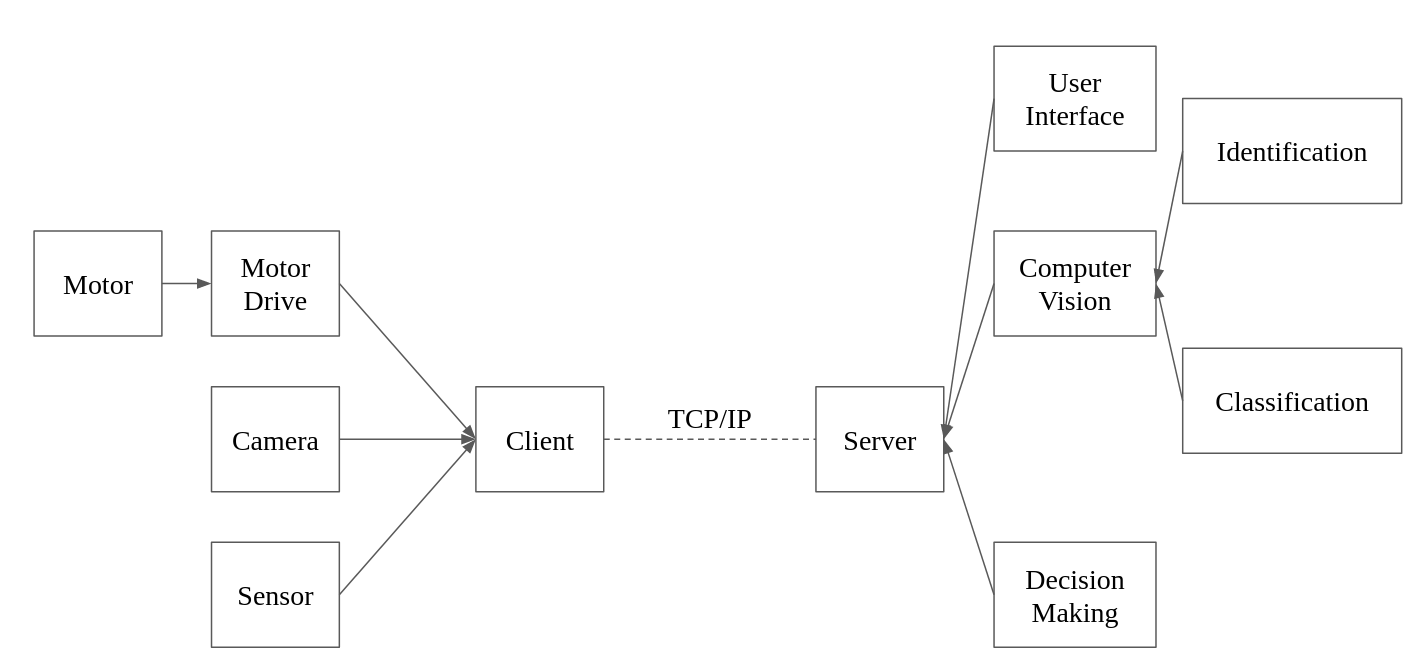
\includegraphics[width=\linewidth]{content/020_overall_design/img/overall_diagram.png}
    \caption{Overall System Parts}
    \label{fig:overall_system_parts}
\end{figure}


This report consists of top down approach which explains the overall description, then diving into smaller parts and sub-parts of them. Overall system description is best demonstrated with the figure in \ref{fig:overall_system_parts}. There are mainly 2 parts, server and client respectively, in addition to the connection between them. Server - client model will be investigated deeper in the \ref{sec:server_client} section with justifications. For now, it is enough to know that the system has 2 parts connected by a computer network implemented over the internet, and these parts have special sub-modules and missions assigned them. System details will be explained in the next sections.

System design is made on requirements and best fits to these requirements. Customer wants, security, safety, as well as technical musts and edge conditions are determined and solutions are developed. A list of requirements for the project is given as below in addition to requirements developed in each component which are specified in the section of the corresponding component.

\begin{itemize}
    \item The product should give response in a few seconds so as not to allow a cat to escape
    \item The product should work for long hours on battery
\end{itemize}

Before going into parts in detail, it is important to make some points clear about the rules and techniques used in the system. Black box approach is the first property each module and team member understands deeply. Each module is seen as black box and each of them can be separated without any loss in functionality. Therefore, any addition from the beginning or a problem that may arise can be solved locally without changing the overall structure of the product and only having a little work since each team member is specialized in the specific part.



%% Tikz stuff...
\tikzstyle{startstop} = [rectangle, text width=0.3\linewidth, minimum width=0.1\linewidth, rounded corners, text centered, draw=black, fill=red!30]
\tikzstyle{io} = [trapezium, trapezium left angle=70, trapezium right angle=110, text centered, draw=black, fill=blue!30]
\tikzstyle{process} = [rectangle, text width=0.4\linewidth, minimum height=0.15\linewidth, text centered, draw=black, fill=orange!30]
\tikzstyle{decision} = [diamond, text width=0.25\linewidth, minimum height=0.2\linewidth, text centered, draw=black, fill=green!30]
\tikzstyle{arrow} = [thick,->,>=stealth]

\begin{wrapfigure}{r}{0.4\textwidth}
\begin{center}
\begin{tikzpicture}[node distance=0.25\linewidth]

%% Nodes...
\node (camera) [startstop] {Camera};
\node (client) [process, below of=camera] {Raspberry Pi};
\node (server) [process, below of=client] {Client};
\node (classifier) [process, below of=server] {Classifier};
\node (topisCatDetected) [draw=none, below of=classifier] {};
\node (isCatDetected) [decision, below of=topisCatDetected] {Cat\\Detected?};
\node (rightisCatDetected) [draw=none, right of=isCatDetected] {};
\node (identifier) [process, text width=0.3\linewidth, right of=rightisCatDetected] {Identifier};
\node (botisCatDetected) [draw=none, below of=isCatDetected] {};
\node (decisionMaker) [process, below of=botisCatDetected] {Decision\\Maker};
\node (takeAction) [startstop, below of=decisionMaker] {Final\\Action};

%% Connections...
\draw[arrow] (camera) -- (client);
\draw[arrow] (client) -- (server);
\draw[arrow] (server) -- (classifier);
\draw[arrow] (classifier) -- (isCatDetected);
\draw[arrow] (isCatDetected) -- node[anchor=east] {no} (decisionMaker);
\draw[arrow] (decisionMaker) -- (takeAction);
\draw[arrow] (isCatDetected) -- node[anchor=north] {yes} (identifier);
\draw[arrow] (identifier) |- (decisionMaker);

\end{tikzpicture}
\end{center}
\caption{Information Flow Chart}
\label{fig:information_flow_chart}
\end{wrapfigure}


Other than system components, information flow and decision making are the two crucial parts of the system. Figure \ref{fig:information_flow_chart} shows how information flows and choice is made by the system. Camera captures the image and it is transferred to the client, Raspberry Pi which is then send through TCP/IP channel to the server side. Server has components to process this information and take action based on the system requirements. The image processor actually consists of two independent phases, classification and identification. Data is processed in classification program which is then sent to identification in case of a cat detected. The cat image is then identified in identification stage with image descriptors. This way, the cat name, or id, is determined and it is returned to the decision control module. Calculations based on database and decision control algorithms, a choice is made. Then the actions are going to be taken.

This design allows better manipulation of data and less computational burden since only specific data, images classified as cats will be exposed to identification process which requires greater computational capability. Moreover, cats can be identified in a few seconds in total so that the system can feed each cat before they quit the scene.

\subsection{Requirements}

\begin{itemize}
    \item \textbf{Computer Vision:}
    \item Differentiate between cats and dogs.
    \item Clearly recognize scenes without any dogs. 
    \item Detect how many cats are present.
    \item Have reliable confidence for the classifications.
    \item \textbf{Electronics:}
    \item The subsystem should be rechargeable and the charging time should be less than 5 hours.
    \item Rechargeable batteries should be non-removable.
    \item Battery duration should be at least 5 hours.
    \item The subsystem should be wired correctly and properly.
    \item The subsystem should be able to operate during charging.
    \item The subsystem should be able to operate Raspberry Pi and Arduino.
    \item The subsystem should be able to drive the servo motor.
    \item Power consumption of the subsystem should be minimum. 
    \item Status of the food supply should be observable.
    \item Battery level for both charging and operation modes should be observable.
    \item The subsystem should be able to measure the amount of given food.
    \item \textbf{Mechanics:}
    \item Total system should be lifted by an ordinary person. 
    \item Volume of the box should be enough for all electronic devices to fit in.
    \item Box should be durable for harsh outdoor conditions.
    \item Food reservoir should be provide at least 100 meals for an ordinary cat.
    \item There should be maximum \%5 waste of food. 
    \item Amount of food remaining, battery chargers while loading and in operation should be visible.
    \item Angle and the position of the camera must be adjusted properly in order to identify cats and dogs from 1.5 meter.
    \item There must be no obstacle in front of the camera unit, so that it can capture accurate photographs.
    \item Camera unit should be adjusted properly so that it should be protected from animal attacks.
\end{itemize}